\section{Support in Score-P and Vampir}

In the following sections the level of support for modern C++ by Score-P and Vampir will be discussed. This is achieved by implementing several small example programs that make use of these features. The source code of these examples can be found in Appendix \ref{app:scorep}. The code is compiled with gcc 6.2.1, using the compiler plugin from Score-P 3.0. The results are examined using Vampir 9.0.

\subsection{Concurrency}\label{scorep:conc}

In this section the various concurrency constructs introduced in C++11 will be discussed.

\subsubsection{\texttt{std::async}}\label{scorep:conc_async}

As mentioned in Section \ref{queue} \texttt{std::async} is a high-level construct to asynchronously run tasks. The underlying management of this asynchronous is not exposed to the library user; instead, it is guaranteed that the result is returned upon a call to \texttt{future::get} (\texttt{std::async} returns a \texttt{std::future}). This may lead to blocking on the caller's side if the asynchronous task has not been completed yet. This potential bottleneck makes any application using \texttt{std::async} a natural target for profiling, even more so as its default behaviour with regard to thread spawning is implementation specific.

There are three test cases in this document: One for the default behaviour (Appendix \ref{app:scorep_conc_async_default}), another for explicit asynchronous evaluation (Appendix \ref{app:scorep_conc_async_async}) and a third for explicit lazy evaluation (Appendix \ref{app:scorep_conc_async_lazy}).

The first two test cases fail with the following error message:

\begin{verbatim}
$ SCOREP_ENABLE_TRACING=1 ./future_default                                      
[Score-P] src/measurement/thread/create_wait/scorep_thread_create_wait
          _pthread.c:84: Fatal: Bug 'tpd == 0': Invalid Pthread thread
          specific data object. Please ensure that all pthread_create
          calls are instrumented.
[Score-P] Please report this to support@score-p.org. Thank you.
[Score-P] Try also to preserve any generated core dumps.
[Score-P] src/measurement/thread/create_wait/scorep_thread_create_wait
          _pthread.c:84: Fatal: Bug 'tpd == 0': Invalid Pthread thread
          specific data object. Please ensure that all pthread_create
          calls are instrumented.[1]    8405 abort (core dumped)
\end{verbatim}

The lazy evaluation test case executes successfully; however, as the code in question is not executed in a separate thread the inspection of Score-P's trace file show nothing of interest (see Figures \ref{scorep:conc_async_lazy_timeline} and \ref{scorep:conc_async_lazy_summary}).

\begin{figure}[htbp]
	\begin{center}
		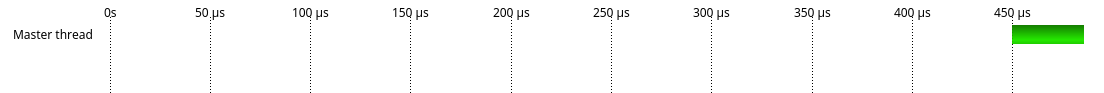
\includegraphics[width=0.9\textwidth]{img/scorep_async_lazy_timeline.png}
		\caption{Timeline for \texttt{std::async} with lazy evaluation}
		\label{scorep:conc_async_lazy_timeline}
	\end{center}
\end{figure}

\begin{figure}[htbp]
	\begin{center}
		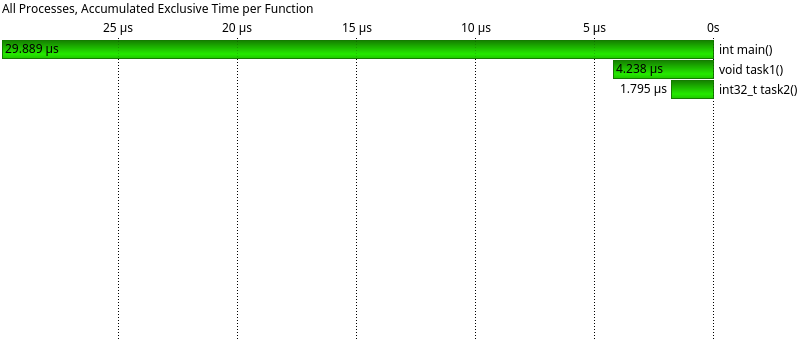
\includegraphics[width=0.9\textwidth]{img/scorep_async_lazy_summary.png}
		\caption{Summary for \texttt{std::async} with lazy evaluation}
		\label{scorep:conc_async_lazy_summary}
	\end{center}
\end{figure}

\subsubsection{\texttt{std::thread}}\label{scorep:conc_thread}

When compared to \texttt{std::async} \texttt{std::thread} follows a much more ``low level'' approach as thread execution is now entirely in the hands of the user. Naturally C++11 threads are profiling targets as well as they build the very foundation of modern C++ style concurrent programming.

There is are two test cases for \texttt{std::thread}: the first spawns a thread and joins it afterwards (Appendix \ref{app:conc_thread_join}), the second spawns a thread and detaches it, making it unjoinable (Appendix \ref{app:conc_thread_detach}).

Both test cases fail to execute and produce the same error message already known from Section \ref{scorep:conc_async}.

\subsubsection{Summary}

At the time of writing, Score-P's support for C++11 multithreading is nonexistent as the error messages from Section \ref{scorep:conc_async} and Section \ref{scorep:conc_thread} show. The likely cause for these errors lies in the internals of the GNU C++ compiler's standard library as the threading support library is compiled into the shared library object. Score-P is unable to instrument this already compiled code and crashes upon execution once it encounters an unknown thread.

The solution for this problem would be a more graceful handling of ``unknown threads'': Instead of crashing Score-P should simply register them on the fly.

\subsection{Synchronization}

With the introduction of the thread support library synchronization primitives were added to the standard library as well. As such primitives are able to block thread execution profiling their behaviour is especially interesting in a HPC context. In this section the mutual exclusion constructs (\texttt{std::mutex}) and condition variables (\texttt{std::condition\_variable}) are evaluated. Due to the problems shown in Section \ref{scorep:conc} the spawned threads in the testcases are classic Pthreads.

\subsubsection{\texttt{std::mutex}}\label{scorep:sync_mutex}

\texttt{std::mutex} and its more specialized siblings \texttt{std::timed\_mutex}, \texttt{std::recursive\_mutex} and \texttt{std::recursive\_timed\_mutex} provide simple mechanisms for mutual exclusion between threads. Like similar primitives these constructs provide mechanisms for locking and unlocking. However, directly accessing these mechanisms is not exception-safe which is why they are usually managed by \texttt{std::unique\_lock} or \texttt{std::lock\_guard}. Relying on \gls{raii} these primitives will automatically unlock the managed \texttt{std::mutex} once they go out of scope.

The test case (see Appendix \ref{app:scorep_sync_mutex}) utilizes them as well for synchronization between two threads instead of locking the \texttt{std::mutex} manually. Upon execution the test case itself works as expected: Pthreads are spawned and \texttt{std::mutex} blocks one of them while being locked by the other.

Score-P on the other hand is not able to fully parse the instruction flow correctly: instead of instrumenting the calls to the standard library facilites it detects and instruments the underlying  Pthread mechanisms utilized by the library implementation (see Figures \ref{scorep:sync_pthread_mutex_timeline} and \ref{scorep:sync_pthread_mutex_summary}). This can be explained by the compiler's aggressive inlining of the \gls{stl} functions which prevents Score-P from instrumenting the actual function call.

\begin{figure}[htbp]
	\begin{center}
		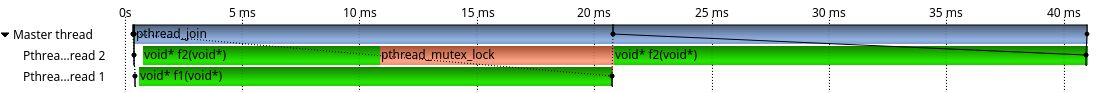
\includegraphics[width=0.9\textwidth]{img/scorep_pthread_mutex_timeline.png}
		\caption{Timeline for thread synchronization with \texttt{std::mutex}}
		\label{scorep:sync_pthread_mutex_timeline}
	\end{center}
\end{figure}

\begin{figure}[htbp]
	\begin{center}
		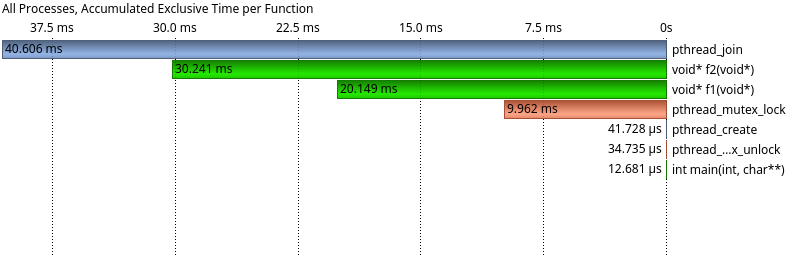
\includegraphics[width=0.9\textwidth]{img/scorep_pthread_mutex_summary.png}
		\caption{Summary for thread synchronization with \texttt{std::mutex}}
		\label{scorep:sync_pthread_mutex_summary}
	\end{center}
\end{figure}

\subsubsection{\texttt{std::condition\_variable}}

The other synchronization primitive added to the standard library with C++11 is \texttt{std::condition\_variable} which allows threads to communicate with each other. A \texttt{std::condition\_variable} is always associated with a \texttt{std::mutex} but offers more fine-grained control via its notification mechanisms -- a thread can either wake up one other waiting thread or all of them.

The test case (see Appendix \ref{app:scorep_sync_cv}) spawns four Pthreads, of which three are waiting for the fourth to signal them. Once they receive the notification they execute their instructions in parallel.

Like the simpler \texttt{std::mutex} test case (see Section \ref{scorep:sync_mutex}) this program executes successfully and suffers from the same problems with inlining (see Figures \ref{scorep:sync_pthread_cv_timeline} and \ref{scorep:sync_pthread_cv_summary}).

\begin{figure}[htbp]
	\begin{center}
		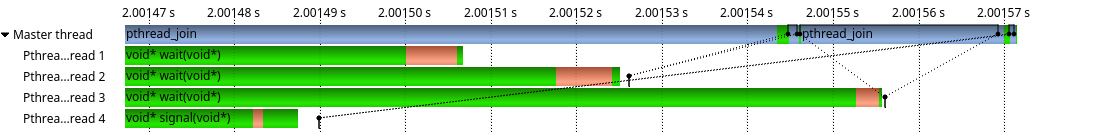
\includegraphics[width=0.9\textwidth]{img/scorep_pthread_cv_timeline.png}
		\caption{Timeline for thread synchronization with \texttt{std::condition\_variable}}
		\label{scorep:sync_pthread_cv_timeline}
	\end{center}
\end{figure}

\begin{figure}[htbp]
	\begin{center}
		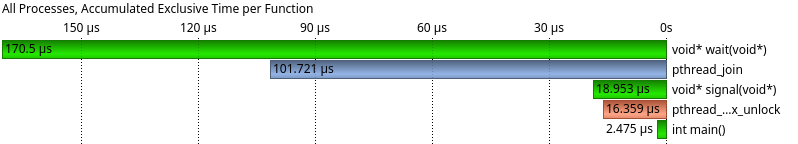
\includegraphics[width=0.9\textwidth]{img/scorep_pthread_cv_summary.png}
		\caption{Summary for thread synchronization with \texttt{std::condition\_variable}}
		\label{scorep:sync_pthread_cv_summary}
	\end{center}
\end{figure}

\subsubsection{Summary}

While Score-P's support for synchronization primitives is better than its support for C++11 threads it is not perfect. Due to aggressive compiler inlining the \gls{stl} functions are optimized away before Score-P can instrument them. Unfortunately, changing this behaviour would be quite hard as this requires either a change to the way instrumentation is currently done or a special codepaths for the \gls{stl} mechanics.